%% bare_conf.tex
%% V1.4b
%% 2015/08/26
%% by Michael Shell
%% See:
%% http://www.michaelshell.org/
%% for current contact information.
%%
%% This is a skeleton file demonstrating the use of IEEEtran.cls
%% (requires IEEEtran.cls version 1.8b or later) with an IEEE
%% conference paper.
%%
%% Support sites:
%% http://www.michaelshell.org/tex/ieeetran/
%% http://www.ctan.org/pkg/ieeetran
%% and
%% http://www.ieee.org/

%%*************************************************************************
%% Legal Notice:
%% This code is offered as-is without any warranty either expressed or
%% implied; without even the implied warranty of MERCHANTABILITY or
%% FITNESS FOR A PARTICULAR PURPOSE! 
%% User assumes all risk.
%% In no event shall the IEEE or any contributor to this code be liable for
%% any damages or losses, including, but not limited to, incidental,
%% consequential, or any other damages, resulting from the use or misuse
%% of any information contained here.
%%
%% All comments are the opinions of their respective authors and are not
%% necessarily endorsed by the IEEE.
%%
%% This work is distributed under the LaTeX Project Public License (LPPL)
%% ( http://www.latex-project.org/ ) version 1.3, and may be freely used,
%% distributed and modified. A copy of the LPPL, version 1.3, is included
%% in the base LaTeX documentation of all distributions of LaTeX released
%% 2003/12/01 or later.
%% Retain all contribution notices and credits.
%% ** Modified files should be clearly indicated as such, including  **
%% ** renaming them and changing author support contact information. **
%%*************************************************************************


% *** Authors should verify (and, if needed, correct) their LaTeX system  ***
% *** with the testflow diagnostic prior to trusting their LaTeX platform ***
% *** with production work. The IEEE's font choices and paper sizes can   ***
% *** trigger bugs that do not appear when using other class files.       ***                          ***
% The testflow support page is at:
% http://www.michaelshell.org/tex/testflow/



\documentclass[conference]{IEEEtran}
\usepackage{graphicx}
\usepackage{float}

% Some Computer Society conferences also require the compsoc mode option,
% but others use the standard conference format.
%
% If has not been installed into the LaTeX system files,
% manually specify the path to it like:
% \documentclass[conference]{../sty/IEEEtran}





% Some very useful LaTeX packages include:
% (uncomment the ones you want to load)


% *** MISC UTILITY PACKAGES ***
%
%\usepackage{ifpdf}
% Heiko Oberdiek's ifpdf.sty is very useful if you need conditional
% compilation based on whether the output is pdf or dvi.
% usage:
% \ifpdf
%   % pdf code
% \else
%   % dvi code
% \fi
% The latest version of ifpdf.sty can be obtained from:
% http://www.ctan.org/pkg/ifpdf
% Also, note that IEEEtran.cls V1.7 and later provides a builtin
% \ifCLASSINFOpdf conditional that works the same way.
% When switching from latex to pdflatex and vice-versa, the compiler may
% have to be run twice to clear warning/error messages.




\usepackage{wrapfig}

% *** CITATION PACKAGES ***
%
\usepackage{cite}
% cite.sty was written by Donald Arseneau
% V1.6 and later of IEEEtran pre-defines the format of the cite.sty package
% \cite{} output to follow that of the IEEE. Loading the cite package will
% result in citation numbers being automatically sorted and properly
% "compressed/ranged". e.g., [1], [9], [2], [7], [5], [6] without using
% cite.sty will become [1], [2], [5]--[7], [9] using cite.sty. cite.sty's
% \cite will automatically add leading space, if needed. Use cite.sty's
% noadjust option (cite.sty V3.8 and later) if you want to turn this off
% such as if a citation ever needs to be enclosed in parenthesis.
% cite.sty is already installed on most LaTeX systems. Be sure and use
% version 5.0 (2009-03-20) and later if using hyperref.sty.
% The latest version can be obtained at:
% http://www.ctan.org/pkg/cite
% The documentation is contained in the cite.sty file itself.






% *** GRAPHICS RELATED PACKAGES ***
%
\ifCLASSINFOpdf
  % \usepackage[pdftex]{graphicx}
  % declare the path(s) where your graphic files are
  % \graphicspath{{../pdf/}{../jpeg/}}
  % and their extensions so you won't have to specify these with
  % every instance of \includegraphics
  % \DeclareGraphicsExtensions{.pdf,.jpeg,.png}
\else
  % or other class option (dvipsone, dvipdf, if not using dvips). graphicx
  % will default to the driver specified in the system graphics.cfg if no
  % driver is specified.
  % \usepackage[dvips]{graphicx}
  % declare the path(s) where your graphic files are
  % \graphicspath{{../eps/}}
  % and their extensions so you won't have to specify these with
  % every instance of \includegraphics
  % \DeclareGraphicsExtensions{.eps}
\fi
% graphicx was written by David Carlisle and Sebastian Rahtz. It is
% required if you want graphics, photos, etc. graphicx.sty is already
% installed on most LaTeX systems. The latest version and documentation
% can be obtained at: 
% http://www.ctan.org/pkg/graphicx
% Another good source of documentation is "Using Imported Graphics in
% LaTeX2e" by Keith Reckdahl which can be found at:
% http://www.ctan.org/pkg/epslatex
%
% latex, and pdflatex in dvi mode, support graphics in encapsulated
% postscript (.eps) format. pdflatex in pdf mode supports graphics
% in .pdf, .jpeg, .png and .mps (metapost) formats. Users should ensure
% that all non-photo figures use a vector format (.eps, .pdf, .mps) and
% not a bitmapped formats (.jpeg, .png). The IEEE frowns on bitmapped formats
% which can result in "jaggedy"/blurry rendering of lines and letters as
% well as large increases in file sizes.
%
% You can find documentation about the pdfTeX application at:
% http://www.tug.org/applications/pdftex





% *** MATH PACKAGES ***
%
\usepackage{amsmath}
% A popular package from the American Mathematical Society that provides
% many useful and powerful commands for dealing with mathematics.
%
% Note that the amsmath package sets \interdisplaylinepenalty to 10000
% thus preventing page breaks from occurring within multiline equations. Use:
%\interdisplaylinepenalty=2500
% after loading amsmath to restore such page breaks as IEEEtran.cls normally
% does. amsmath.sty is already installed on most LaTeX systems. The latest
% version and documentation can be obtained at:
% http://www.ctan.org/pkg/amsmath





% *** SPECIALIZED LIST PACKAGES ***
%
\usepackage{algorithmic}
% algorithmic.sty was written by Peter Williams and Rogerio Brito.
% This package provides an algorithmic environment fo describing algorithms.
% You can use the algorithmic environment in-text or within a figure
% environment to provide for a floating algorithm. Do NOT use the algorithm
% floating environment provided by algorithm.sty (by the same authors) or
% algorithm2e.sty (by Christophe Fiorio) as the IEEE does not use dedicated
% algorithm float types and packages that provide these will not provide
% correct IEEE style captions. The latest version and documentation of
% algorithmic.sty can be obtained at:
% http://www.ctan.org/pkg/algorithms
% Also of interest may be the (relatively newer and more customizable)
% algorithmicx.sty package by Szasz Janos:
% http://www.ctan.org/pkg/algorithmicx




% *** ALIGNMENT PACKAGES ***
%
%\usepackage{array}
% Frank Mittelbach's and David Carlisle's array.sty patches and improves
% the standard LaTeX2e array and tabular environments to provide better
% appearance and additional user controls. As the default LaTeX2e table
% generation code is lacking to the point of almost being broken with
% respect to the quality of the end results, all users are strongly
% advised to use an enhanced (at the very least that provided by array.sty)
% set of table tools. array.sty is already installed on most systems. The
% latest version and documentation can be obtained at:
% http://www.ctan.org/pkg/array


% IEEEtran contains the IEEEeqnarray family of commands that can be used to
% generate multiline equations as well as matrices, tables, etc., of high
% quality.




% *** SUBFIGURE PACKAGES ***
%\ifCLASSOPTIONcompsoc
%  \usepackage[caption=false,font=normalsize,labelfont=sf,textfont=sf]{subfig}
%\else
%  \usepackage[caption=false,font=footnotesize]{subfig}
%\fi
% subfig.sty, written by Steven Douglas Cochran, is the modern replacement
% for subfigure.sty, the latter of which is no longer maintained and is
% incompatible with some LaTeX packages including fixltx2e. However,
% subfig.sty requires and automatically loads Axel Sommerfeldt's caption.sty
% which will override IEEEtran.cls' handling of captions and this will result
% in non-IEEE style figure/table captions. To prevent this problem, be sure
% and invoke subfig.sty's "caption=false" package option (available since
% subfig.sty version 1.3, 2005/06/28) as this is will preserve IEEEtran.cls
% handling of captions.
% Note that the Computer Society format requires a larger sans serif font
% than the serif footnote size font used in traditional IEEE formatting
% and thus the need to invoke different subfig.sty package options depending
% on whether compsoc mode has been enabled.
%
% The latest version and documentation of subfig.sty can be obtained at:
% http://www.ctan.org/pkg/subfig




% *** FLOAT PACKAGES ***
%
%\usepackage{fixltx2e}
% fixltx2e, the successor to the earlier fix2col.sty, was written by
% Frank Mittelbach and David Carlisle. This package corrects a few problems
% in the LaTeX2e kernel, the most notable of which is that in current
% LaTeX2e releases, the ordering of single and double column floats is not
% guaranteed to be preserved. Thus, an unpatched LaTeX2e can allow a
% single column figure to be placed prior to an earlier double column
% figure.
% Be aware that LaTeX2e kernels dated 2015 and later have fixltx2e.sty's
% corrections already built into the system in which case a warning will
% be issued if an attempt is made to load fixltx2e.sty as it is no longer
% needed.
% The latest version and documentation can be found at:
% http://www.ctan.org/pkg/fixltx2e


%\usepackage{stfloats}
% stfloats.sty was written by Sigitas Tolusis. This package gives LaTeX2e
% the ability to do double column floats at the bottom of the page as well
% as the top. (e.g., "\begin{figure*}[!b]" is not normally possible in
% LaTeX2e). It also provides a command:
%\fnbelowfloat
% to enable the placement of footnotes below bottom floats (the standard
% LaTeX2e kernel puts them above bottom floats). This is an invasive package
% which rewrites many portions of the LaTeX2e float routines. It may not work
% with other packages that modify the LaTeX2e float routines. The latest
% version and documentation can be obtained at:
% http://www.ctan.org/pkg/stfloats
% Do not use the stfloats baselinefloat ability as the IEEE does not allow
% \baselineskip to stretch. Authors submitting work to the IEEE should note
% that the IEEE rarely uses double column equations and that authors should try
% to avoid such use. Do not be tempted to use the cuted.sty or midfloat.sty
% packages (also by Sigitas Tolusis) as the IEEE does not format its papers in
% such ways.
% Do not attempt to use stfloats with fixltx2e as they are incompatible.
% Instead, use Morten Hogholm'a dblfloatfix which combines the features
% of both fixltx2e and stfloats:
%
% \usepackage{dblfloatfix}
% The latest version can be found at:
% http://www.ctan.org/pkg/dblfloatfix




% *** PDF, URL AND HYPERLINK PACKAGES ***
%
%\usepackage{url}
% url.sty was written by Donald Arseneau. It provides better support for
% handling and breaking URLs. url.sty is already installed on most LaTeX
% systems. The latest version and documentation can be obtained at:
% http://www.ctan.org/pkg/url
% Basically, \url{my_url_here}.




% *** Do not adjust lengths that control margins, column widths, etc. ***
% *** Do not use packages that alter fonts (such as pslatex).         ***
% There should be no need to do such things with IEEEtran.cls V1.6 and later.
% (Unless specifically asked to do so by the journal or conference you plan
% to submit to, of course. )

\usepackage{subcaption}
\usepackage[utf8]{inputenc}
\hyphenation{op-tical net-works semi-conduc-tor}
\DeclareMathOperator*{\argminA}{arg\,min} % Jan Hlavacek

\begin{document}
%
% paper title
% Titles are generally capitalized except for words such as a, an, and, as,
% at, but, by, for, in, nor, of, on, or, the, to and up, which are usually
% not capitalized unless they are the first or last word of the title.
% Linebreaks \\ can be used within to get better formatting as desired.
% Do not put math or special symbols in the title.
\title{Fundamental Mapping from Relational Database to MongoDB}

% author names and affiliations
% use a multiple column layout for up to three different
% affiliations
\author{\IEEEauthorblockN{Tuan Dung Lai}
\IEEEauthorblockA{Faculty of Science, Engineering and Technology\\
Swinburne University of Technology\\
Hawthorn, Victoria 3122\\
Email: tuandunglai@gmail.com}}

% conference papers do not typically use \thanks and this command
% is locked out in conference mode. If really needed, such as for
% the acknowledgment of grants, issue a \IEEEoverridecommandlockouts
% after \documentclass

% for over three affiliations, or if they all won't fit within the width
% of the page, use this alternative format:
% 
%\author{\IEEEauthorblockN{Michael Shell\IEEEauthorrefmark{1},
%Homer Simpson\IEEEauthorrefmark{2},
%James Kirk\IEEEauthorrefmark{3}, 
%Montgomery Scott\IEEEauthorrefmark{3} and
%Eldon Tyrell\IEEEauthorrefmark{4}}
%\IEEEauthorblockA{\IEEEauthorrefmark{1}School of Electrical and Computer Engineering\\
%Georgia Institute of Technology,
%Atlanta, Georgia 30332--0250\\ Email: see http://www.michaelshell.org/contact.html}
%\IEEEauthorblockA{\IEEEauthorrefmark{2}Twentieth Century Fox, Springfield, USA\\
%Email: homer@thesimpsons.com}
%\IEEEauthorblockA{\IEEEauthorrefmark{3}Starfleet Academy, San Francisco, California 96678-2391\\
%Telephone: (800) 555--1212, Fax: (888) 555--1212}
%\IEEEauthorblockA{\IEEEauthorrefmark{4}Tyrell Inc., 123 Replicant Street, Los Angeles, California 90210--4321}}




% use for special paper notices
%\IEEEspecialpapernotice{(Invited Paper)}




% make the title area
\maketitle

% As a general rule, do not put math, special symbols or citations
% in the abstract
\begin{abstract}
NoSQL database are becoming a fundamental role of the database landscape nowadays, first version released in 2007, at that time, MySQL, an open-source relational database management system (RDBMS) has been developed extensively for more than 10 years. NoSQL has a handful of advantages including lower cost, easier scalability and open sources features. However, NoSQL is still a relatively young technology, making it difficult for  IT engineer and student to learn.
\end{abstract}

% no keywords




% For peer review papers, you can put extra information on the cover
% page as needed:
% \ifCLASSOPTIONpeerreview
% \begin{center} \bfseries EDICS Category: 3-BBND \end{center}
% \fi
%
% For peerreview papers, this IEEEtran command inserts a page break and
% creates the second title. It will be ignored for other modes.
\IEEEpeerreviewmaketitle


\section{Introduction}
With the less constrained structure, scalable schema design of NoSQL and faster access compared to traditional RDBMS. Coming from an SQL background, it could be challenging and time-consuming to map database management concept from SQL to NoSQL. This report will go through fundamental concept of MongoDB functionality, terms and simple query syntax. The difference of this report is that we assume that you have basic knowledge of SQL, and everything from this report will be built and map based on that knowledge you have on SQL.
\section{Mapping Tables, Rows, Columns}
\subsection{Quick SQL review}
In SQL databse, tables are objects that are being managed, all data or information of objects and database are stored in tables. Table contains column (a set of data values of a particular type) and row (attribute type and their value). The columns provide the structure according to which the rows are composed.
\subsection{Collection}
Each database in MongoDB consists of collections which are equivalent to an RDBMS database consisting of SQL tables.
Collection stores data in the form of documents which is equivalent to tables storing data in rows.
\begin{center}
 \begin{tabular}{||c c||} 
 \hline
   SQL & NoSQL  \\ [0.5ex] 
 \hline\hline
 Table & Collection  \\ 
 \hline
 Column & JSON structure   \\
 \hline
 Row & Field\\
 [1ex] 
 \hline
\end{tabular}
\end{center}
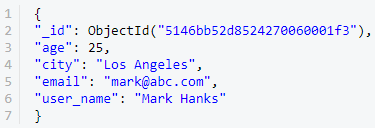
\includegraphics{collection}
The document above is equivalent to a row in RDBMS, a collection contains multiple document above. This document use JSON format, it consists of key value pairs.
\\
Notice that the field above has a unique id. It is considered as primary key when comparing to MySQL.
\begin{figure}[H]
    \centering
    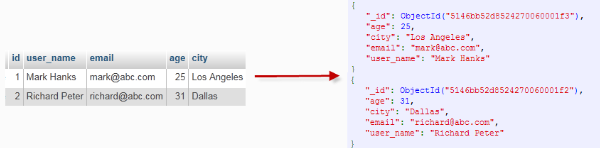
\includegraphics[width=10cm]{collection_mapping}
    \caption{Mapping table to collection~\cite{4}}
    \label{fig:fig4}
\end{figure}
\subsection{Dynamic Schema}
In NoSQL, documents within a collection can have different schema. The fields in MongoDB can be easily added, removed and modified. For example, typical documents have 4 fields, like students have name, class, gender and date of birth, now, it is possible to create a student that have name, faculty and parent details. The number of fields as well as structure can be different. There is no constraint on data types of the fields. This functionality to use dynamic schema allows us to generate dynamic documents at run time.

For instance, consider the following two documents inside the same collection but having different schemas (Fig 2):
\begin{figure}[H]
    \centering
    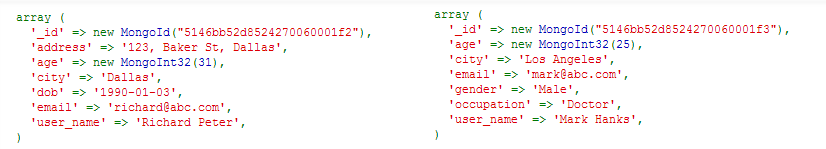
\includegraphics[width=10cm]{dynamicshema}
    \caption{Dynamic schema example~\cite{4}}
    \label{fig:fig4}
\end{figure}
The first document contains the fields address and dob which are not present in the second document while the second document contains fields gender and occupation which are not present in the first one. Imagine if we would have designed this thing in SQL, we would have kept four extra columns for address, dob, gender and occupation, some of which would store empty (or null) values, and hence occupying unnecessary space.

This model of dynamic schema is the reason why NoSQL databases are highly scalable in terms of design. Various complex schemas (hierarchical, tree-structured, etc) which would require number of RDBMS tables can be designed efficiently using such documents. A typical example would be to store user posts, their likes, comments and other associated information in the form of documents. An SQL implementation for the same would ideally have separate tables for storing posts, comments and likes while a MongoDB document can store all these information in a single document.
\section{Mapping Join and Relationships}
\subsection{Quick SQL review}
Relationships in RDBMS are achieved using primary and foreign key relationships and querying those using joins. There is no such straightforward mapping in MongoDB but the relationships here are designed using embedded and linking documents.
\begin{figure}[H]
    \centering
    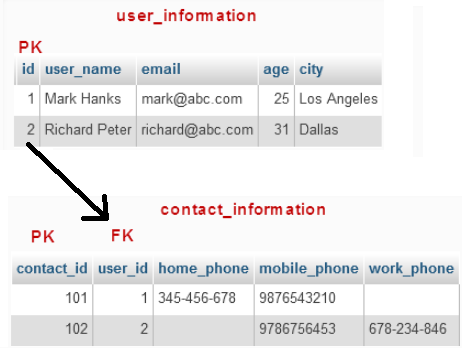
\includegraphics[width=8cm]{pfkf}
    \caption{Relation in SQL}
    \label{fig:fig4}
\end{figure}

\indent
\subsection{Linking Documents and Embedding Documents}
\subsubsection{Linking Documents}
Linking documents is a method in which multiple collections are created with some similar fields both collection, these similar fields are equivalent to foreign key in SQL.
\begin{figure}[H]
    \centering
    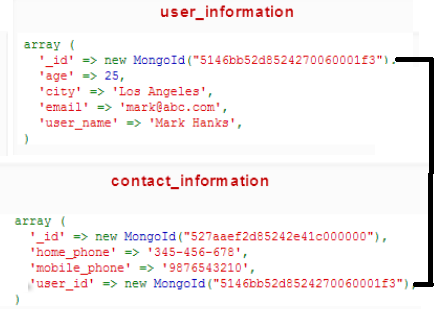
\includegraphics[width=8cm]{linkingdocuments}
    \caption{Linking Document in NoSQL}
    \label{fig:fig4}
\end{figure}
The user id field in our document in Fig 4 is simply a field that holds some data and all the logic associated with it has to be implemented by us. For example, even if you will insert some user id in the contact information document that does not exist in the user information collection, MongoDB is not going to throw any error saying that corresponding user id was not found in the user information collection(unlike SQL where this would be an invalid foreign key constraint).
\subsubsection{Embedding Documents}
Embedding documents mean instead of creating separate collections as we did in Linking Document, we will try to merge every information into one collection. The fields that are being copied from one collection to another collection will be extended in only one collection.
\begin{figure}[H]
    \centering
    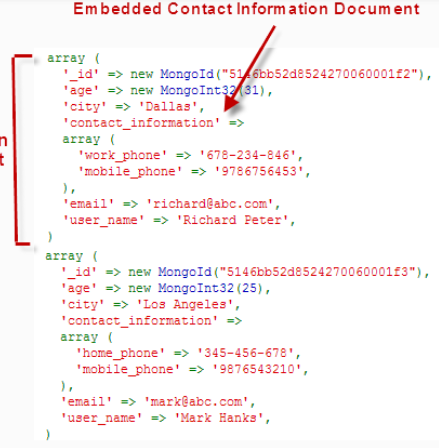
\includegraphics[width=8cm]{embeddeddocuments}
    \caption{Embedded Documents  in NoSQL}
    \label{fig:fig4}
\end{figure}
In the above example, we have embedded a small document of contact information inside the user information. In the similar manner, large complex documents and hierarchical data can be embedded like this to relate entities.
\section{Mapping Query}
In this section, we will translate all fundamental query from MySQL to MongoDB along with example in syntax.
Let's start with a brief on terminology and concepts:
\begin{center}
 \begin{tabular}{||c c||} 
 \hline
   SQL & NoSQL  \\ [0.5ex] 
 \hline\hline
 database & database  \\ 
 \hline
 table & 	collection   \\
 \hline
 row & document or JSON document \\
  \hline
 column & 		field   \\
  \hline
 index & 		index   \\
  \hline
 table joins & 	lookup, embedded documents   \\
  \hline
 primary key & 	 primary key   \\
   \hline
 aggregation  & aggregation pipeline   \\
 [1ex] 
 \hline
\end{tabular}
\end{center}
\subsection{Create}
In MongoDB, it is not possible and not necessary to define the structure of a collection as we normally did in MySQL (create table, naming column, define data type). MongoDB use JSON format which is an unstructured format to store data.\\
The structure of the document is automatically created when the first insert occurs in the collection. However, you can create an empty collection using createCollection command.
\begin{figure}[H]
    \centering
    \includegraphics[width=8cm]{createsql}
    \caption{Create table in SQL}
    \label{fig:fig4}
\end{figure}
In MongoDB, we can only create an empty collection:
\begin{center}
\textbf{\textit{db.createCollection("posts")}}.
\end{center}
\subsection{Insert}
\begin{figure}[H]
    \centering
    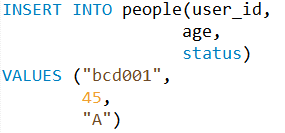
\includegraphics[width=6cm]{insertsql}
    \caption{Insert data in SQL}
    \label{fig:fig4}
\end{figure}
Data in NoSQL has JSON format, we can either insert the JSON file to collection or insert key-value pair into collection.
\begin{center}
\textbf{\textit{db.people.insert(
   { userid: "bcd001", age: 45, status: "A" }
)}}.
\end{center}
Note: We can create a new field for id. However, The inserted document will contain the auto generated id field.
\subsection{Read}
\subsubsection{Read All Data}
MongoDB uses the find method which is equivalent to the SELECT command in SQL. The following statements simply read all the documents from the posts collection.
\begin{figure}[H]
    \centering
    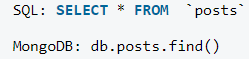
\includegraphics[width=6cm]{read1}
    \caption{Read all data}
    \label{fig:fig4}
\end{figure}
\subsubsection{Read specific data in collection}
The following query fetches specific columns, post text  and post likes count as specified in the second set of braces {}. We mark the value as 1 in the second bracket to include the field in the output.
\begin{figure}[H]
    \centering
    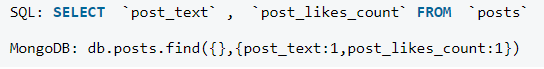
\includegraphics[width=9cm]{read2}
    \caption{Read specific data}
    \label{fig:fig4}
\end{figure}
\subsubsection{Read data with condition}
The following query does a conditional search for documents having username field as mark. All the criteria for fetching the documents have to be placed in the first braces {} separated by commas.
\begin{figure}[H]
    \centering
    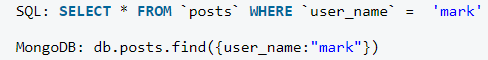
\includegraphics[width=9cm]{read3}
    \caption{Read data with condition}
    \label{fig:fig4}
\end{figure}
\subsubsection{Read auto generate ID}
In MongoDB, every time we input new data, one specific id will be auto generated and this id will be displayed by all read commands that we described above. Set id to 0 to disable showing id with find command.

\begin{center}
\textbf{\textit{db.posts.find({},{posttext:1,postlikescount:1,id:0})}}.
\end{center}
\subsubsection{Read specific data with condition}
\begin{figure}[H]
    \centering
    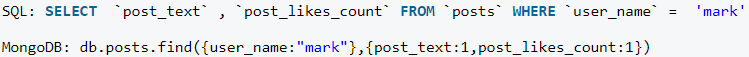
\includegraphics[width=10cm]{read4}
    \caption{Read specific data with condition}
    \label{fig:fig4}
\end{figure}
\subsubsection{Logical Operator}
We will examine how to do an \textbf{OR} operator in MongoDB, same syntax applied to other logical operators.
\begin{figure}[H]
    \centering
    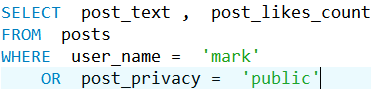
\includegraphics[width=7cm]{orsql}
    \caption{Logical operator OR in MySQL}
    \label{fig:fig4}
\end{figure}
In MongoDB, we use the following command:
\begin{center}
\textbf{\textit{db.posts.find({\$or:[{username:'mark'},{postprivacy: 'public'}]},{posttext:1,postlikescount:1})})}.
\end{center}
\subsubsection{Sort}

Next, we will use the sort method which sorts the result in ascending order of postlikescount(indicated by 1).
\begin{figure}[H]
    \centering
    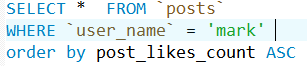
\includegraphics[width=7cm]{sortsql}
    \caption{Sort in MySQL}
    \label{fig:fig4}
\end{figure}
\begin{center}
\textbf{\textit{db.posts.find({username:"mark"}).sort({postlikescount:1})})}.
\end{center}
To sort the results in descending order,  we specify -1 as the value of the field.
\begin{center}
\textbf{\textit{db.posts.find({username:"mark"}).sort({postlikescount:-1})})}.
\end{center}
\subsubsection{Limit display output data}
To limit the number of documents to be returned, we use the limit method specifying the number of documents.
\begin{figure}[H]
    \centering
    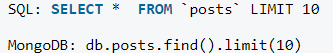
\includegraphics[width=7cm]{Limit}
    \caption{Limit number of output data being displayed}
    \label{fig:fig4}
\end{figure}
\subsection{Update}
The first parameter to the update method specifies the criteria to select the documents. The second parameter specifies the actual update operation to be performed. For example, the following query selects all the documents with username as mark and sets their postprivacy as private.\\
One difference here is that by default, MongoDB update query updates only one (and the first matched) document. To update all the matching documents we have to provide a third parameter specifying multi as true indicating that we want to update multiple documents.
\\\\
\textbf{\textit{db.posts.update({username:"mark"},{\$set:{postprivacy:"private"\\}},{multi:true})}}.

\begin{figure}[H]
    \centering
    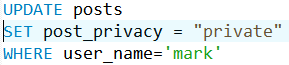
\includegraphics[width=6cm]{updatesql}
    \caption{Update in SQL}
    \label{fig:fig4}
\end{figure}

\subsection{Remove}
\begin{figure}[H]
    \centering
    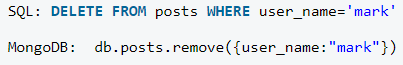
\includegraphics[width=9cm]{remove}
    \caption{Remove comparison}
    \label{fig:fig4}
\end{figure}
\section{Conclusion}
This report has shown you fundamental concept of MongoDB, most of the core concepts in term of data management are similar to MySQL. Upon this report, reader should try out more complex queries such as map reduce in order to gain more knowledge of NoSQL.\\
Attached to this report is an example where the author of this report convert an University database in SQL to NoSQL. Reader can check out that report for further details.

\section*{Acknowledgment}
The author would like to thank Dr. Irene Moser, my lecture for the unit called Fundamental of Data Management, unit code COS20015. She has provided a great series of useful lecture which help me a lot in term of understanding data management theory. Also, I would like to thank my tutor Rasoul Rahmani for great support during the semester.
\indent

\begin{thebibliography}{5}

\bibitem{1}
https://docs.microsoft.com/en-us/sql/relational-databases/tables/primary-and-foreign-key-constraints

\bibitem{2}
https://www.javatpoint.com/mongodb-history

\bibitem{3}
https://code.tutsplus.com/articles/mapping-relational-databases-and-sql-to-mongodb--net-35650

\bibitem{4}
https://docs.mongodb.com/manual/reference/sql-comparison/

\bibitem{5}
https://docs.microsoft.com/en-us/sql/relational-databases/tables/create-foreign-key-relationships

\end{thebibliography}
\end{document}


